\documentclass{article}
\usepackage[final]{nips_2016} % produce camera-ready copy
% if you need to pass options to natbib, use, e.g.:
\PassOptionsToPackage{numbers, compress}{natbib}
% before loading nips_2016
%
% % to avoid loading the natbib package, add option nonatbib:
% \usepackage[nonatbib]{nips_2016}

% \usepackage{nips_2016}

% % to compile a camera-ready version, add the [final] option, e.g.:
% \usepackage[final]{nips_2016}

\usepackage[utf8]{inputenc} % allow utf-8 input
\usepackage[T1]{fontenc}    % use 8-bit T1 fonts
\usepackage{hyperref}       % hyperlinks
\usepackage{url}            % simple URL typesetting
\usepackage{booktabs}       % professional-quality tables
\usepackage{amsfonts}       % blackboard math symbols
\usepackage{nicefrac}       % compact symbols for 1/2, etc.
\usepackage{microtype}      % microtypography
\usepackage{amsmath}
\usepackage{mathtools}
\title{Deep Learning Assignment 4}

% The \author macro works with any number of authors. There are two
% commands used to separate the names and addresses of multiple
% authors: \And and \AND.
%
% Using \And between authors leaves it to LaTeX to determine where to
% break the lines. Using \AND forces a line break at that point. So,
% if LaTeX puts 3 of 4 authors names on the first line, and the last
% on the second line, try using \AND instead of \And before the third
% author name.
\author{
  Peter Yun-shao Sung
  \texttt{yss265@nyu.edu} \\
  %% examples of more authors
  %% \AND
  %% Coauthor \\
  %% Affiliation \\
  %% Address \\
  %% \texttt{email} \\
  %% \And
  %% Coauthor \\
  %% Affiliation \\
  %% Address \\
  %% \texttt{email} \\
  %% \And
  %% Coauthor \\
  %% Affiliation \\
  %% Address \\
  %% \texttt{email} \\
}

\begin{document}
% \nipsfinalcopy is no longer used

\maketitle
\section{Approaches to RNN}
\subsection{Architecture}
The initial model is based on lstm as building block, with 2 layers and 20 sequence length. Layers are horizontally considering the current given input (or word) and the states passed from previous sequence. Sequence is the stack of multiple layers, and is used for vertically passing states to the next layers. This way, model can not only predict the next word based on current word (horizontal), but the predictions can be altered based on the sequence of previous words (vertical). Regarding to each lstm layer, there are number of rnn\_size lstm unit, and each of the unit perform the operation shown as figure 1.

\begin{figure}[h]
\centering
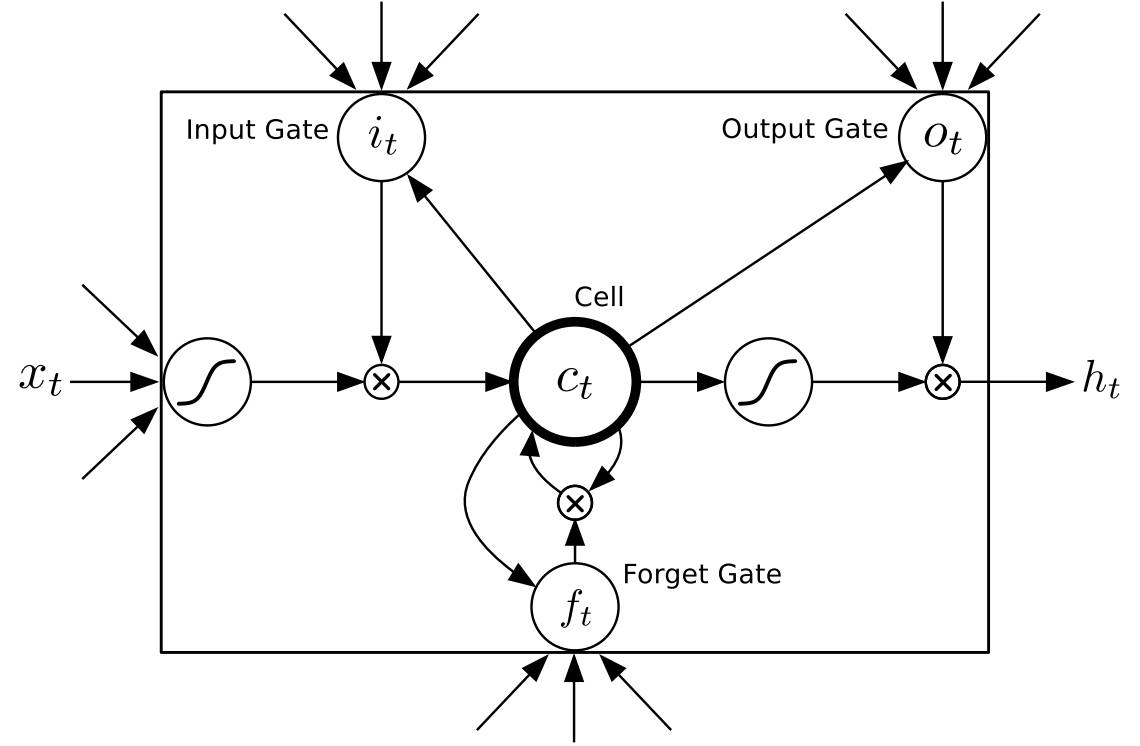
\includegraphics[width=50mm]{./fig/lstm.png}
  \caption{Operation of each of lstm unit}
\end{figure}

\subsection{Learning Techniques}
The two main learning techniques were the dropout and gradient clip. Dropout method was applied between each of lstm module and the final output. The inital module didnot used the dropout, and therefore we can observed that the perplexity of training improved well but not for the validation. This implies the concerns of overfitting and dropout might be a good option to improve.\\
Gradient clipping might be important method during the learning process too. Soft-clipping was initially applied to the model, which it observes the L2 norm of gradient and every gradient will multiply the portions it overpassed if the norm is higher than the threshold. The other method I used during this assignment is hard clipping, which we only cut the gradiend for only the one that pass threshold, instead of the every gradients. The inspiration is mainly from the curiousity of whether soft clipping downgrade the learning process for other gradient.

\subsection{Training Procedure}
Data was preprocessed in the shape of (lines,batch\_size), which is basically to traing a batch size of words. During each forward or backward propagation, line $i$ and $i+1$ is the corresponding current and next word. When feed in network, the $next\_h$ is the output from the lstm module which is in the shape of (batch\_size, vocab\_size), and further calculates the prediction of each word along the batch\_size axis by LogSoftMax. The perplexity is the accumulated error calculated by ClassNLLCriterion, and we are optimizing the perplexity error metric.


\section{Softmax regression gradient calculation}


\end{document}






